\documentclass{article}
\usepackage[backend=bibtex]{biblatex}
\usepackage[margin=1in]{geometry}
\usepackage{amsmath}
\usepackage{amssymb}
\usepackage{graphicx}
\bibliography{references} % the name of your .bib bibliography file, without the file extension

% some helpful math commands I like to define
\newcommand{\vect}[1]{\ensuremath{\mathbf{#1}}}
\newcommand{\mat}[1]{\ensuremath{\mathbf{#1}}}
\newcommand{\transpose}{\ensuremath{\mathsf{T}}}
\newcommand{\of}[1]{\ensuremath{\left(#1\right)}}

% document information
\title{Status Update}
\author{Kyle Volle}
\date{\today} % or put in a fixed date (e.g. 12 June 2014) if you want it to stay put

\begin{document}
\maketitle

%\begin{abstract}
%If you want an abstract, put it here. Otherwise delete this section including the \verb|%\begin{abstract}| and \verb|\end{abstract}| tags.
%\end{abstract}

\section{Research}

This research looks at entirely decentralized cooperation for multi-agent systems in hazardous or even antagonistic environments. In particular, it looks at a situation in which a team of aerial weapons have a set of targets and the agents must autonomously partition themselves into sub-teams that each collectively engage a certain target from the set. 

This project encompasses several sub-problems, some of which are being investigated concurrently and others represent future work. These problems include decentralized clustering, communication across sparse networks, simultaneous location and mapping, mapping of hazards in the environment, path planning and synchronization of effort by the agents.

To date, most of the work has been focused on decentralized clustering. This problem can be framed in a number of ways depending on the solution being implemented. The first method investigated was Markov Decision Processes, in particular Partially-Observable Markov Decision Processes (POMDPs).

In the POMDP formulation, an agent's state is a tuple with the first term being the target currently assigned to it and the rest of the terms being the number of agents assigned to each target.  POMDPs also require a transition function that describes the results of actions. Since the actions are not entirely deterministic and communication ranges are limited the world state is only partially observable, otherwise the problem could be reduced to just a Markov decision process. However belief states can be created based on most likely results of actions and what sensor information is available and assign probability distributions to these belief states. Finally, POMDPs require a reward function that is a function of the state and corresponds to how desirable being in that state is. Solving a POMDP returns an optimal policy which gives the best action to take in a given belief state.

The downside of POMDPs is that the state space can quickly grow intractable and use up large amounts of memory and take too long for practical purposes, particularly for value iteration. In fact, if unreachable states are not culled, the state space for this problem with $n$ weapons and $t$ targets has $t\left(n+1\right)^{t}$ states. However more thoughtful methods of enumerating states can reduce this by almost two orders of magnitude. If mission details are known in advance, the optimal policy can be calculated offline and distributed to the agents in advance. Making the assumption that the model used to generate the policy is sufficiently close to the ground truth, the policy generated will be close to the optimal policy for the actual situation. This policy can be input into the policy iteration algorithm to make minor corrections on the fly.

POMDPs showed promise in a simplified version of the problem but quickly became intractable as the state space grew when more realistic models were fleshed out. In simulations of the simplified problem each agent needed to make only one change of target decision in order for the state of the entire system to converge to a global optimum. Unfortunately POMDPs work best with discrete valued states and factoring in bearing and range to each target, as well as weapon effectiveness and attrition rates, added too many continuous valued states for the problem to be tractable.

Another method investigated over the past few weeks has been simulated annealing. With this approach, if an agent is in an undesirable state it has a non-zero probability at each time step of taking an action that would move it to another state. This action is selected randomly based on a probability distribution across all possible actions with the probability based on the desirability of the state that would result. Since agents in desirable states have zero probability of changing their state, eventually the algorithm will converge to an optimal state. This approach has the advantage of requiring much less information about the global state than POMDPs and it also requires no pre-planning. The trade-off is that it sacrifices a guarantee of optimality for a probabilistic guarantee.

To evaluate a state, the kill probability (Pk) on each target is needed. Each agent has a Pk for each target based on the type of target, size of the weapon and the attrition rate over the path from the agent to the target. The Pk for a target is the amalgamation of the Pk's for that target of each agent currently targeting it. The relative priority of each target can be expressed by the desired Pk for that target. For example a high priority target might have a desired Pk of 0.99 whereas a lower priority target might have a Pk of 0.55. The total difference between the current Pks and desired Pks gives us a way to compare the desirability of two states. In the example below, 150 agents are targeting 30 targets of varying priority. The average difference between the current and desired Pks is plotted in Figure \ref{fig:avg_err}.

\begin{figure}[h]
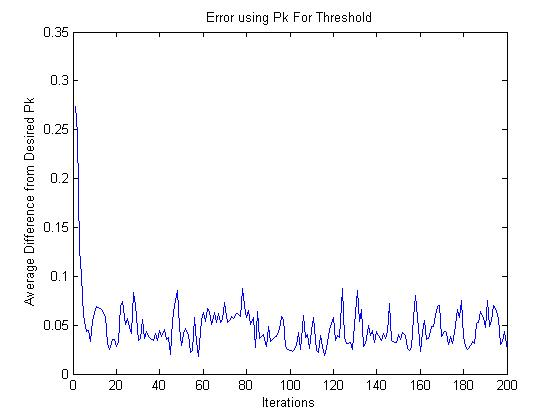
\includegraphics[width=1\textwidth]{avg_err}
\caption{Simulated Annealing Trial Run}
\label{fig:avg_err}
\end{figure}

\section{Pathfinder Project}

For the Pathfinder Project, a quadrotor simulator was implemented in Matlab. The simulator takes forces and moments in the body-fixed reference frame and calculates the values of the vehicle state at the next time step based on 12 coupled differential equations. The simulator was parameterized so that by just changing a few variables different vehicles such as the AR.Drone and 3DR Quad can be simulated.

The simulator also includes simulated sensors that take the truth values as calculated by the simulator and add in sensor noise and sensor biases. The amount of noise and bias for each sensor is based on the results of tests done with the hardware. This allows for testing the robustness of the control system to sensor noise as well as for testing the state estimator being designed in parallel with the controller.

A nested PID controller was integrated with the simulation. The controller takes as inputs desired velocities and calculates the commanded thrust for each motor. By doing this in simulation first it allows the control structure to be validated and for gains to be tuned before the controller is implemented on the hardware. The performance of this controller can be seen in Figure \ref{fig:control}.

\begin{figure}[h]
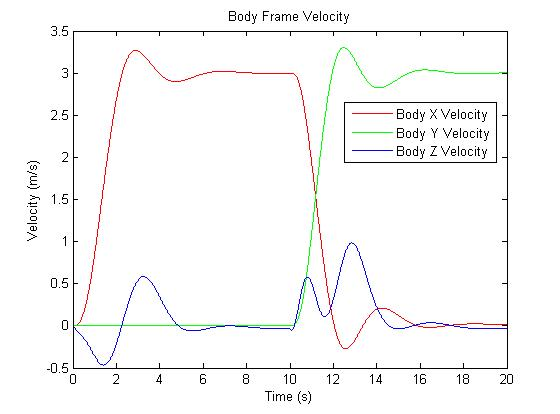
\includegraphics[width=1\textwidth]{control}
\caption{Response to step changes in velocity}
\label{fig:control}
\end{figure}

For an additional layer of verification, the controller was implemented in ROS so that it could be interfaced with the Gazebo simulation environment. A quadrotor simulation for Gazebo developed at Darmstadt Technical University is being used to test the controller.

The next step is to run this control system on the PX4 in flight. Initially, it will be run parallel with the existing control system to ensure that the motor commands it generates are reasonable and appropriate. Assuming that no issues arise, it will then completely replace the existing PX4 controller.

Additionally, I've been working with Chau Ton on implementing a sliding mode controller for a quadrotor as part of his research.

\printbibliography

\end{document}